%!TEX root = ../template.tex
%%%%%%%%%%%%%%%%%%%%%%%%%%%%%%%%%%%%%%%%%%%%%%%%%%%%%%%%%%%%%%%%%%%%
%% implementation.tex
%% NOVA thesis document file
%%
%% Chapter with lots of dummy text
%%%%%%%%%%%%%%%%%%%%%%%%%%%%%%%%%%%%%%%%%%%%%%%%%%%%%%%%%%%%%%%%%%%%
\chapter{Device design and implementation }
\label{cha:device_design}


% Device design
% Introduction
This section commences with an analysis of the available options, the inherent limitations that were identified, and other significant considerations related to the implementation of this project. Subsequently, the specifications of the system implemented in this dissertation will be described, along with the rationale behind the decisions made during the implementation phase.
This process cannot be conducted without first acknowledging the constraints imposed by the unique circumstances of this particular case. The first of these constraints is financial, as the absence of external funding significantly reduces the range of available options. Furthermore, the options for suitable hardware are constrained by their compatibility with the essential free and open-source software that will be utilized in the project. The software in question is of critical importance in meeting the necessary criteria for the system to be considered as vehicular.
In the majority of cases of this nature, the issue of performance is also a significant concern. The capabilities of the components of the device are of significant importance when considering the performance of our solution, as they directly impact the device’s performance. However, our main goal is to demonstrate the feasibility of such a device, and as such it is necessary to set aside concerns regarding performance in order to reduce the cost.
In the event that any of the aforementioned restrictions prove to be applicable, they will be duly noted in the appropriate section.
% Box design
\section{Architectural design}

This section delineates the design decisions that were implemented in the process of assembling the device, in accordance with the architecture of the \gls{sdn} layers.

% Data plane
\subsection{Data plane}

This subsection offers a comprehensive overview of the data plane's fundamental components, encompassing its hardware elements, \gls{os}, wireless communication strategies, and virtualized switching programs.

% Hardware components 
\subsubsection{Hardware components}
The selection of appropriate hardware was guided by the different categories of \gls{sdn} devices outlined in section~\ref{subsec:control_plane}. Accordingly, our analysis began with an assessment of the viability of each of the three proposed approaches for the intended implementation of the solution resulting from this project. In light of these criteria and of the existing financial restrictions, general-purpose hardware emerged as the optimal choice for this problem, largely due to its comparatively lower cost. The proposed implementation will be based on the use of general-purpose hardware, with the switching functions being emulated through the use of software.
% General purpose computers
The process of assembling any device requires attention to the individual components that will be incorporated and that comprise the complete system. The most notable components include the motherboard, the \gls{cpu}, the \gls{ram}, the \gls{nic}, the power supply, and the case. It should be noted that a multitude of additional components could be considered, given that, in real world development, an \gls{obu} is often equipped with a plethora of other specialized dongles.
The selection of the motherboard exerts a determining influence on the subsequent choice of other components; therefore, it became the starting point. Following an exhaustive review of a multitude of products from various corporations in all the methodologies identified, the products from two companies have emerged from the comprehensive research conducted. These solutions have been identified as sufficient candidates for addressing the specific challenges in our case study.
\begin{itemize}
    \item PC Engines~\cite{noauthor_pc_nodate}: 
    PC Engines boards are designed for use in academic institutions and for networking purposes. The company provides not motherboards, but complete affordable solutions, which include \gls{cpu}, \gls{ram}, \gls{nic}, power supply, and case. Additionally, these solutions rely on active cooling, which facilitates their assembly and reduces operational costs. Another notable feature is the number of ethernet ports and the quantity of \gls{pci} slots, which are both sufficient for the intended use. Lastly, other projects at this university have utilized boards from this company.
    \item Raspberry Pi~\cite{ltd_buy_nodate}: 
    Raspberry Pi is a very well known series of small single-board computers developed by the Raspberry Pi Foundation in association with Broadcom. As a highly recognizable brand, it offers comprehensive assistance and is a well-established brand with a substantial code and user base. This solution's main strength lies in its modularity, as the hardware can be assembled in accordance with specific requirements, thereby allowing for a high degree of flexibility and adaptability. These components are mostly inexpensive, which presents a valuable upside when considering deployment.
\end{itemize}
From these two options, and given the established familiarity, the PC Engines option stands as the most appropriate choice. As stated above, PC Engines' boards are sold as integrated solutions, comprising a pre-selected range of components. The decision regarding the specific model to be adopted from this company will consequently have a significant impact on a multitude of other components. The exact model that will be deployed will be discussed in detail at a later stage. 
In regard to the potential utilization of dongles in a real-world development setting, it is evident that the device would be equipped with a multitude of sensors intended to gather diverse types of data and enhance the device's capabilities. This work will primarily focus on a proof of concept for the integration of the communication component of \glspl{vanet} with \gls{sdn} principles. Consequently, further discussion of the sensors used in vehicles will be omitted. The only noteworthy dongle that we will be employing are bidirectional wireless devices capable of communication at 6GHz.

% OS
\subsubsection{\glsxtrlong{os}}
Having completed the analysis of the hardware, the appropriate next step is to proceed with the examination of the software. The foundation of any software architecture stack is the \gls{bios} of the system. It is thus fitting to initiate this analysis at this level. In a context where specific switching hardware had been selected, the \gls{bios} of the system would assume a greater significance. In this particular scenario, it would be reasonable to consider the potential use of Open Network Install Environment~\cite{noauthor_deploy_nodate}, an open and free standard specifically designed for these use cases. However, given that we will be employing general-purpose hardware, there is no compatibility with such software, and we are therefore effectively compelled to utilize the \gls{bios} that is natively integrated into the motherboard.
The \gls{os} is installed on top of the \gls{bios}, and thus, this discussion will proceed with an examination of the extant options for the \gls{os}. Once more, in the event that we were to utilize switching hardware, \gls{onl}, Stratum or \gls{sonic} would be optimal choices. Stratum, \gls{onl} and \gls{sonic} are open-source \glspl{os} designed for use with switch hardware. Given that we intend to utilize generic hardware, any compatible Linux-based \gls{os} is an adequate option.

% Wireless communication
\subsubsection{Wireless communication}
Our research is focused on achieving wireless communication in vehicular environments. To this end, it must be ensured that the machine is able to communicate using one or both of the \gls{ieee} 802.11p and \gls{c-v2x} standards. It would be very beneficial for the device to be capable of communicating with \gls{lte} and 5G networks; given the time constraints, the priority for this device is the ability to communicate in the \gls{ieee} 802.11p standard.
As one descends through the hierarchical structure of the \gls{etsi} standards for vehicular communication, it becomes increasingly challenging for \gls{sdn} technologies to adapt and conform to existing standards. All layers above the link layer can be readily modified or altered using \gls{sdn} technologies in a manner that allows them to be considered vehicular. The \gls{ieee} 802.11p standard, which represents the lowest level of the stack, is not as straightforward as other layers. Our research revealed three distinct methods for enabling it:
\begin{itemize}
    \item Purpose made hardware: The first option is to acquire specialized hardware that is capable of communicating at the desired frequency while complying with the necessary standards. This solution is the most straightforward, but also the most expensive. Consequently, for the same reasons as for the rest of the hardware, this option is the most viable solution and will not be considered further.
    \item Driver patch: Some researchers have solved this problem~\cite{noauthor_httpsgitlabcomhpi-potsdamosmg5--linux11p--linuxid14_nodate} by employing the use of a capable chipset and modifying the diver code to enable communication in the desired manner. This approach has been previously implemented in other research projects at this institution, and as such the first box received for use in this project is already equipped with this patch.
    This solution is especially appealing because it is the most affordable. However, it is also the most complex solution, as the implementation of such a feat requires a comprehensive understanding of networking, the \gls{ieee} 802.11p standard, drivers, and kernel modules. Even with this knowledge, a chip that is capable of communicating at the desired frequencies and with an open-source device driver for linux systems is required.

    The intricate nature of this component renders the development of a solution from scratch an arduous and time-consuming process, which is impractical within the context of this project. Fortunately, as previously stated, there is existing research that can be utilized to achieve this goal. In a similar context, this university has previously employed a patch for an atheros chip. This family of chips operates with open-source drivers, of which the driver in question is named "ath9k."
    One factor that merits attention is the age of this driver. The ath9k driver is designed for \gls{ieee} 802.11n, which was released in 2009, and raises concerns about its long-term reliability. Furthermore, there appears to be no initiative within the community to implement this solution on modern drivers, nor to make the existing implementations official~\cite{noauthor_ath10k_2023}. 
    \item \gls{sdr}: \gls{sdr} is a relatively recent technology which bears resemblance to \gls{sdn}. It enables the user to modify and configure radio signals. In comparison to the preceding option, this appears to be a more long-term solution, albeit at a higher price point. The subject of \gls{sdr} research is beyond the scope of this dissertation, and therefore it will not be a topic of discussion.
\end{itemize}

Of the three options presented, the most promising is the utilization of an Atheros chip in conjunction with the existing patch. Should this approach prove inadequate, it will be necessary to consider one of the alternative strategies.

% Virtualized switch program
\subsubsection{Virtualized switch program}
The selected hardware type mandates the use of software to emulate the typical functionality of a switch. The implementation of this methodology is contingent upon the availability of virtualized switch software. Our research has identified two potential options: \gls{ovs}~\cite{noauthor_open_nodate-3} and \gls{bmv2}~\cite{noauthor_p4langbehavioral-model_nodate}.
\gls{ovs} is an open-source implementation of a distributed virtual multilayer switch, designed with the intention of providing a switching stack for hardware virtualization environments. In contrast, \gls{bmv2} is a pure \gls{p4} software switch, which is primarily utilized as a testing tool for the \gls{p4} language. Both options are available as free software, but it should be noted that \gls{ovs} is not merely an OpenFlow switch. Consequently, it is significantly more utilized than \gls{bmv2} and offers considerably broader support.
In this study, we will evaluate both solutions to ascertain their capabilities and viability within the context of our conceptual framework.

% Southbound API
\subsection[Southbound API]{Southbound \gls{api}}

The decision regarding the southbound \gls{api} is unambiguous and will be made in accordance with the established conventions within this field. Accordingly, tests will be conducted on both OpenFlow and \gls{p4}Runtime. In regard to the question of the gNXI stack, its role is not indispensable for demonstrating the research question, and thus it will be set aside for the purposes of this study. While the value of integrating gNXI in communication is of great importance in real deployments, this study aims to prioritize the establishment of communication, and thus the integration of such systems will be considered secondary. 

% Control plane
\subsection{Control plane}

Generally, each controller framework comes with its own properties, features and characteristics. The choice of what controller is best for a network is dependent on performance and compatibility.  As previously stated, the issue of performance is not a significant concern in this particular context. In regard to compatibility, the term denotes the ability of the controller framework to operate in conjunction with a multitude of different technologies. This is not a cause for concern since the lower layers utilize open and industry-standard protocols and software, which are universally adopted.
It is currently not feasible to integrate \gls{sdn} software with Vanetza, OpenC2X, or other software that emulates the \gls{its} stack. Additionally, none of the controllers currently available offer support for the standardized \gls{vanet} protocols, necessitating a comprehensive redesign of the system.
When all factors are considered, the choice of control technology is ultimately a matter of preference. Smida et al.~\cite{smida_efficient_2020} compared the performance of four of the most popular controllers in an \gls{sdvn} environment. These were Pythonic Network Operating System, Floodlight, OpenDaylight and \gls{onos}. The article concludes that the best performing controller framework is \gls{odl}, although the results demonstrated that \gls{onos}, Floodlight, and \gls{odl} exhibited comparable performance when a minimal number of vehicles were involved. In light of the aforementioned stipulations, any of the aforementioned controllers would be an adequate choice. In the absence of a sufficiently compelling argument to make any of the aforementioned controllers the superior choice, the decision was made to select \gls{onos}~\cite{noauthor_opennetworkinglabonos_nodate}.


% Northbound API and Application plane
\subsection[Northbound API and Application plane]{Northbound \gls{api} and Application plane}

The choice of either the Northbound \gls{api} or the Application plane is inconsequential, as it is entirely contingent upon the specific controller in question. Moreover, the present study will concentrate on the lower layers.

% Box 1
\section{Box implementation: version 1}
\label{sec:box_v1}


To initiate the practical component of this dissertation, a fully operational device was received consisting of a PC Engines apu1d4 motherboard, containing an AMD G-series T40E \gls{cpu} and 4 GB of \gls{dram}. The device also possesses three Realtek RTL8111E Gigabit Ethernet channels, a DB9 serial port, and two external USBs. Beyond these features, the device is equipped with two \gls{mpcie} interfaces and one \gls{msata} interface. 
These specifications, along with more specific details, were sourced from the product page and are presented as follows:

\begin{itemize}
    \item \gls{cpu}: The device has an AMD G-series T40E, operating at a frequency of 1 GHz. It is comprised of two Bobcat cores, each of which is dual-threaded and capable of supporting 64-bit instructions. Each core has 32K of data, 32K of instructions, and 512K of level 2 cache.
    \item \gls{ram}: 4 GB of DDR3-1066 \gls{dram}
    \item Storage: the device may be booted from an \gls{sd} card connected via USB, an external USB drive, or a \gls{msata} \gls{ssd}. The system's \gls{msata} interface is equipped with the requisite power connector for the \gls{ssd} to function.
    \item Power supply: the device consumes approximately 6 to 12 W at 12 V DC, with the exact value depending on the \gls{cpu} load. The jack is 2.5 mm and center positive.
    \item Connectivity: The device features three Gigabit Ethernet channels, which are Realtek RTL8111E.
    \item Input/Output: The device features a DB9 serial port, four USB ports (two external and two internal), three front panel LEDs, and a pushbutton.
    \item Expansion: The device features two \gls{mpcie} slots, one of which is equipped with a \gls{sim} socket. 
    \item Size: The board measures 152.4 x 152.4 mm. The box that encompasses it totals 15.7 cm x 16.8 cm x 2.7 cm, or 16.7 cm x 18.8 cm x 3 cm when all extremities are included.
    \item Firmware: As part of its low-level system initialization, this device relies on the Coreboot firmware.
    \item Cooling: A conductive cooling system is employed, whereby the \gls{cpu} and south bridge are connected to the enclosure via a 3 mm aluminum heat spreader.
\end{itemize}


The apparatus was furnished with a 16 GB \gls{ssd}, a Compex WLE200NX \gls{mpcie} card for WiFi, and another specialized card for \gls{lte}, which is not germane to our present discussion. To support the necessary functionality of the aforementioned cards, the device was also fitted with four pigtail cables. The assembled device can be seen on Figure~\ref{fig:device_1}.

\begin{figure}
	\centering
	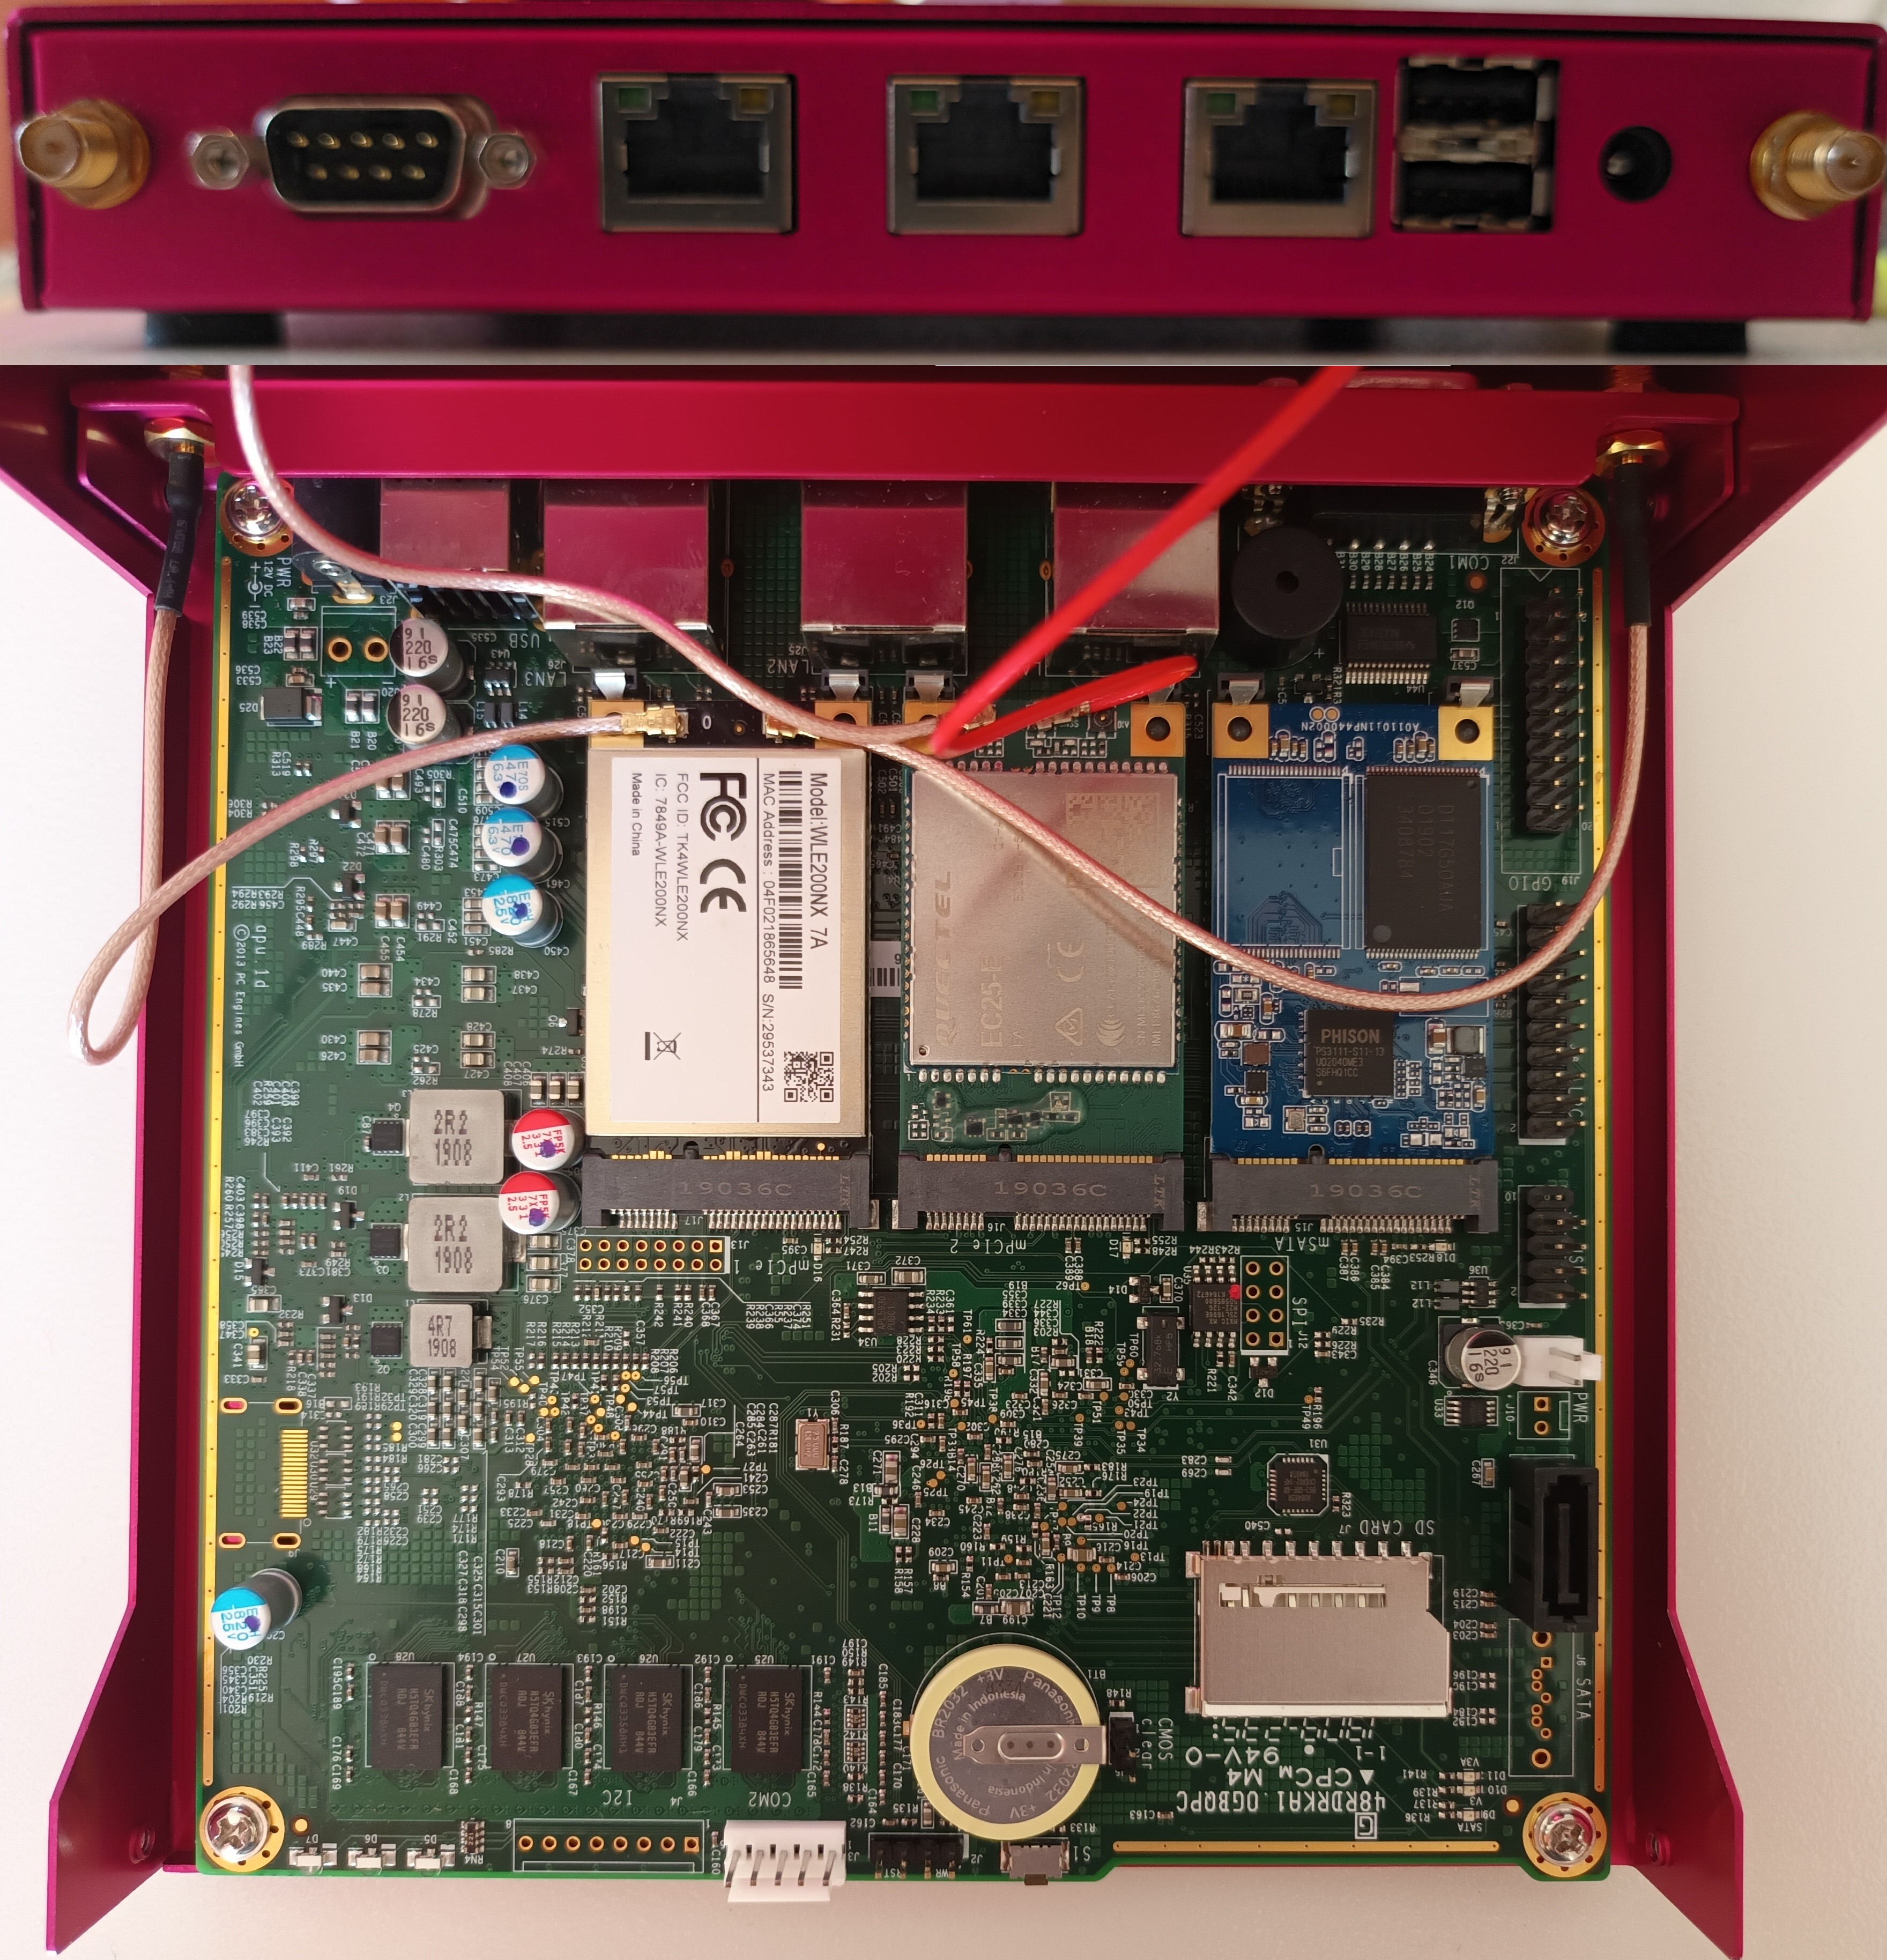
\includegraphics[width=\textwidth]{Chapters/Figures/Implementation/devices/device_1.jpg}
	\caption{Back and inside view from device version 1}
	\label{fig:device_1}
\end{figure}

The device runs on the Debian 12 \gls{os} and has been previously configured to enable communication in the capacity of an \gls{obu}/\gls{its} vehicle station.
The inaugural stage of implementation aimed to ascertain the feasibility of the proposed approach and identify potential avenues for further exploration. It was thus deemed appropriate to commence with an examination of the switching software. The original intention was to install \gls{ovs} and \gls{bmv2} on the aforementioned device and test their compatibility with the existing software. However, this plan was promptly halted due to the device's lack of the necessary resources for installing both programs, and as such we were compelled to deploy \gls{ovs} exclusively on this device. 
A series of tests was conducted to evaluate its capabilities, utilizing both a local controller and a remote \gls{onos} controller. The limited capabilities of the devices also motivated us to opt against installing local controllers on each device. This is contrary to our \gls{sdn} vision, but it is a consequence of the constraints on resources. Another noteworthy obstacle encountered was the insufficient number of test units, which hindered the assessment of the system's wireless communication capabilities between multiple units with a controller.

% Box 2
\section{Box implementation: version 2}
\label{sec:box_v2}

The dearth of a sufficient number of devices for testing halted our progress. In light of these circumstances, the procurement of one or more supplementary devices became imperative. To that end, work began with the aim to to design, and subsequently assemble, two new prototype devices with enhanced specifications.
Two recently constructed prototypes were assembled on a PC Engines apu3d4 motherboard. The motherboard in question is equipped with an AMD G-Series GX-412TC Embedded processor, 4 GB of \gls{dram}, three Intel i211AT Gigabit Ethernet channels, a DB9 serial port, and two external USB 3.0 ports. The device is additionally equipped with three \gls{mpcie} slots, one of which is also capable of functioning as a \gls{msata}. 
These specifications, along with more specific details, were sourced from the product page and are presented as follows:

\begin{itemize}
    \item \gls{cpu}: The device is equipped with an AMD Embedded G-Series GX-412TC, operating at a frequency of 1 GHz. It comprises quad Jaguar cores with 64-bit processing and AES-NI support. Each core has 32 KB of L1 data cache, 32 KB of L1 instruction cache, and a shared 2 MB L2 cache.
    \item \gls{ram}: 4 GB of DDR3-1333 \gls{dram}
    \item Storage: The device may be booted from an \gls{sd} card, an external USB connection, or an \gls{msata} \gls{ssd}. The system's \gls{msata} interface is furnished with the necessary power connector for the \gls{ssd} to operate, and it can also function as an \gls{mpcie} interface.
    \item Power supply: the device consumes approximately 6 to 12 W at 12 V DC, with the exact value depending on the \gls{cpu} load. The jack is 2.5 mm and center positive.
    \item Connectivity: The device features three Gigabit Ethernet channels, which are Intel i211AT.
    \item Input/Output: The device features a DB9 serial port, two USB 3.0 external ports, and four USB 2.0 internal ports. Additionally, it exhibits three front panel LEDs and a pushbutton.
    \item Expansion: The device is equipped with three \gls{mpcie} slots. Of the aforementioned slots, one is a USB or \gls{msata} slot that can accommodate a \gls{sim} card. The second is a USB-only slot that can also accept a \gls{sim} card. The final slot is a full \gls{mpcie} slot, devoid of a \gls{sim} card, but equipped with a WiFi module.
    \item Size: The board measures 152.4 x 152.4 mm. The box that encompasses it totals 15.7 cm x 16.8 cm x 2.7 cm, or 16.7 cm x 16.8 cm x 3 cm when all extremities are included.
    \item Firmware: As part of its low-level system initialization, this device relies on the Coreboot firmware.
    \item Cooling: A conductive cooling system is employed, whereby the \gls{cpu} is connected to the enclosure via a 3 mm aluminum heat spreader.
\end{itemize}

The device was outfitted with a Kingston 256GB \gls{ssd}, a Compex WLE9000VX 7AA WiFi card, and a Quectel EC25-E for \gls{lte}. The prototype case under consideration is only capable of accommodating two pigtail cables. In consideration of our intention to utilize WiFi exclusively for the duration of our investigation, this case is deemed sufficient. Nevertheless, should \gls{lte} be required in the future, enhancements to the case will be mandatory. One of the two newly assembled devices can be seen on figure~\ref{fig:device_2}.

\begin{figure}
	\centering
	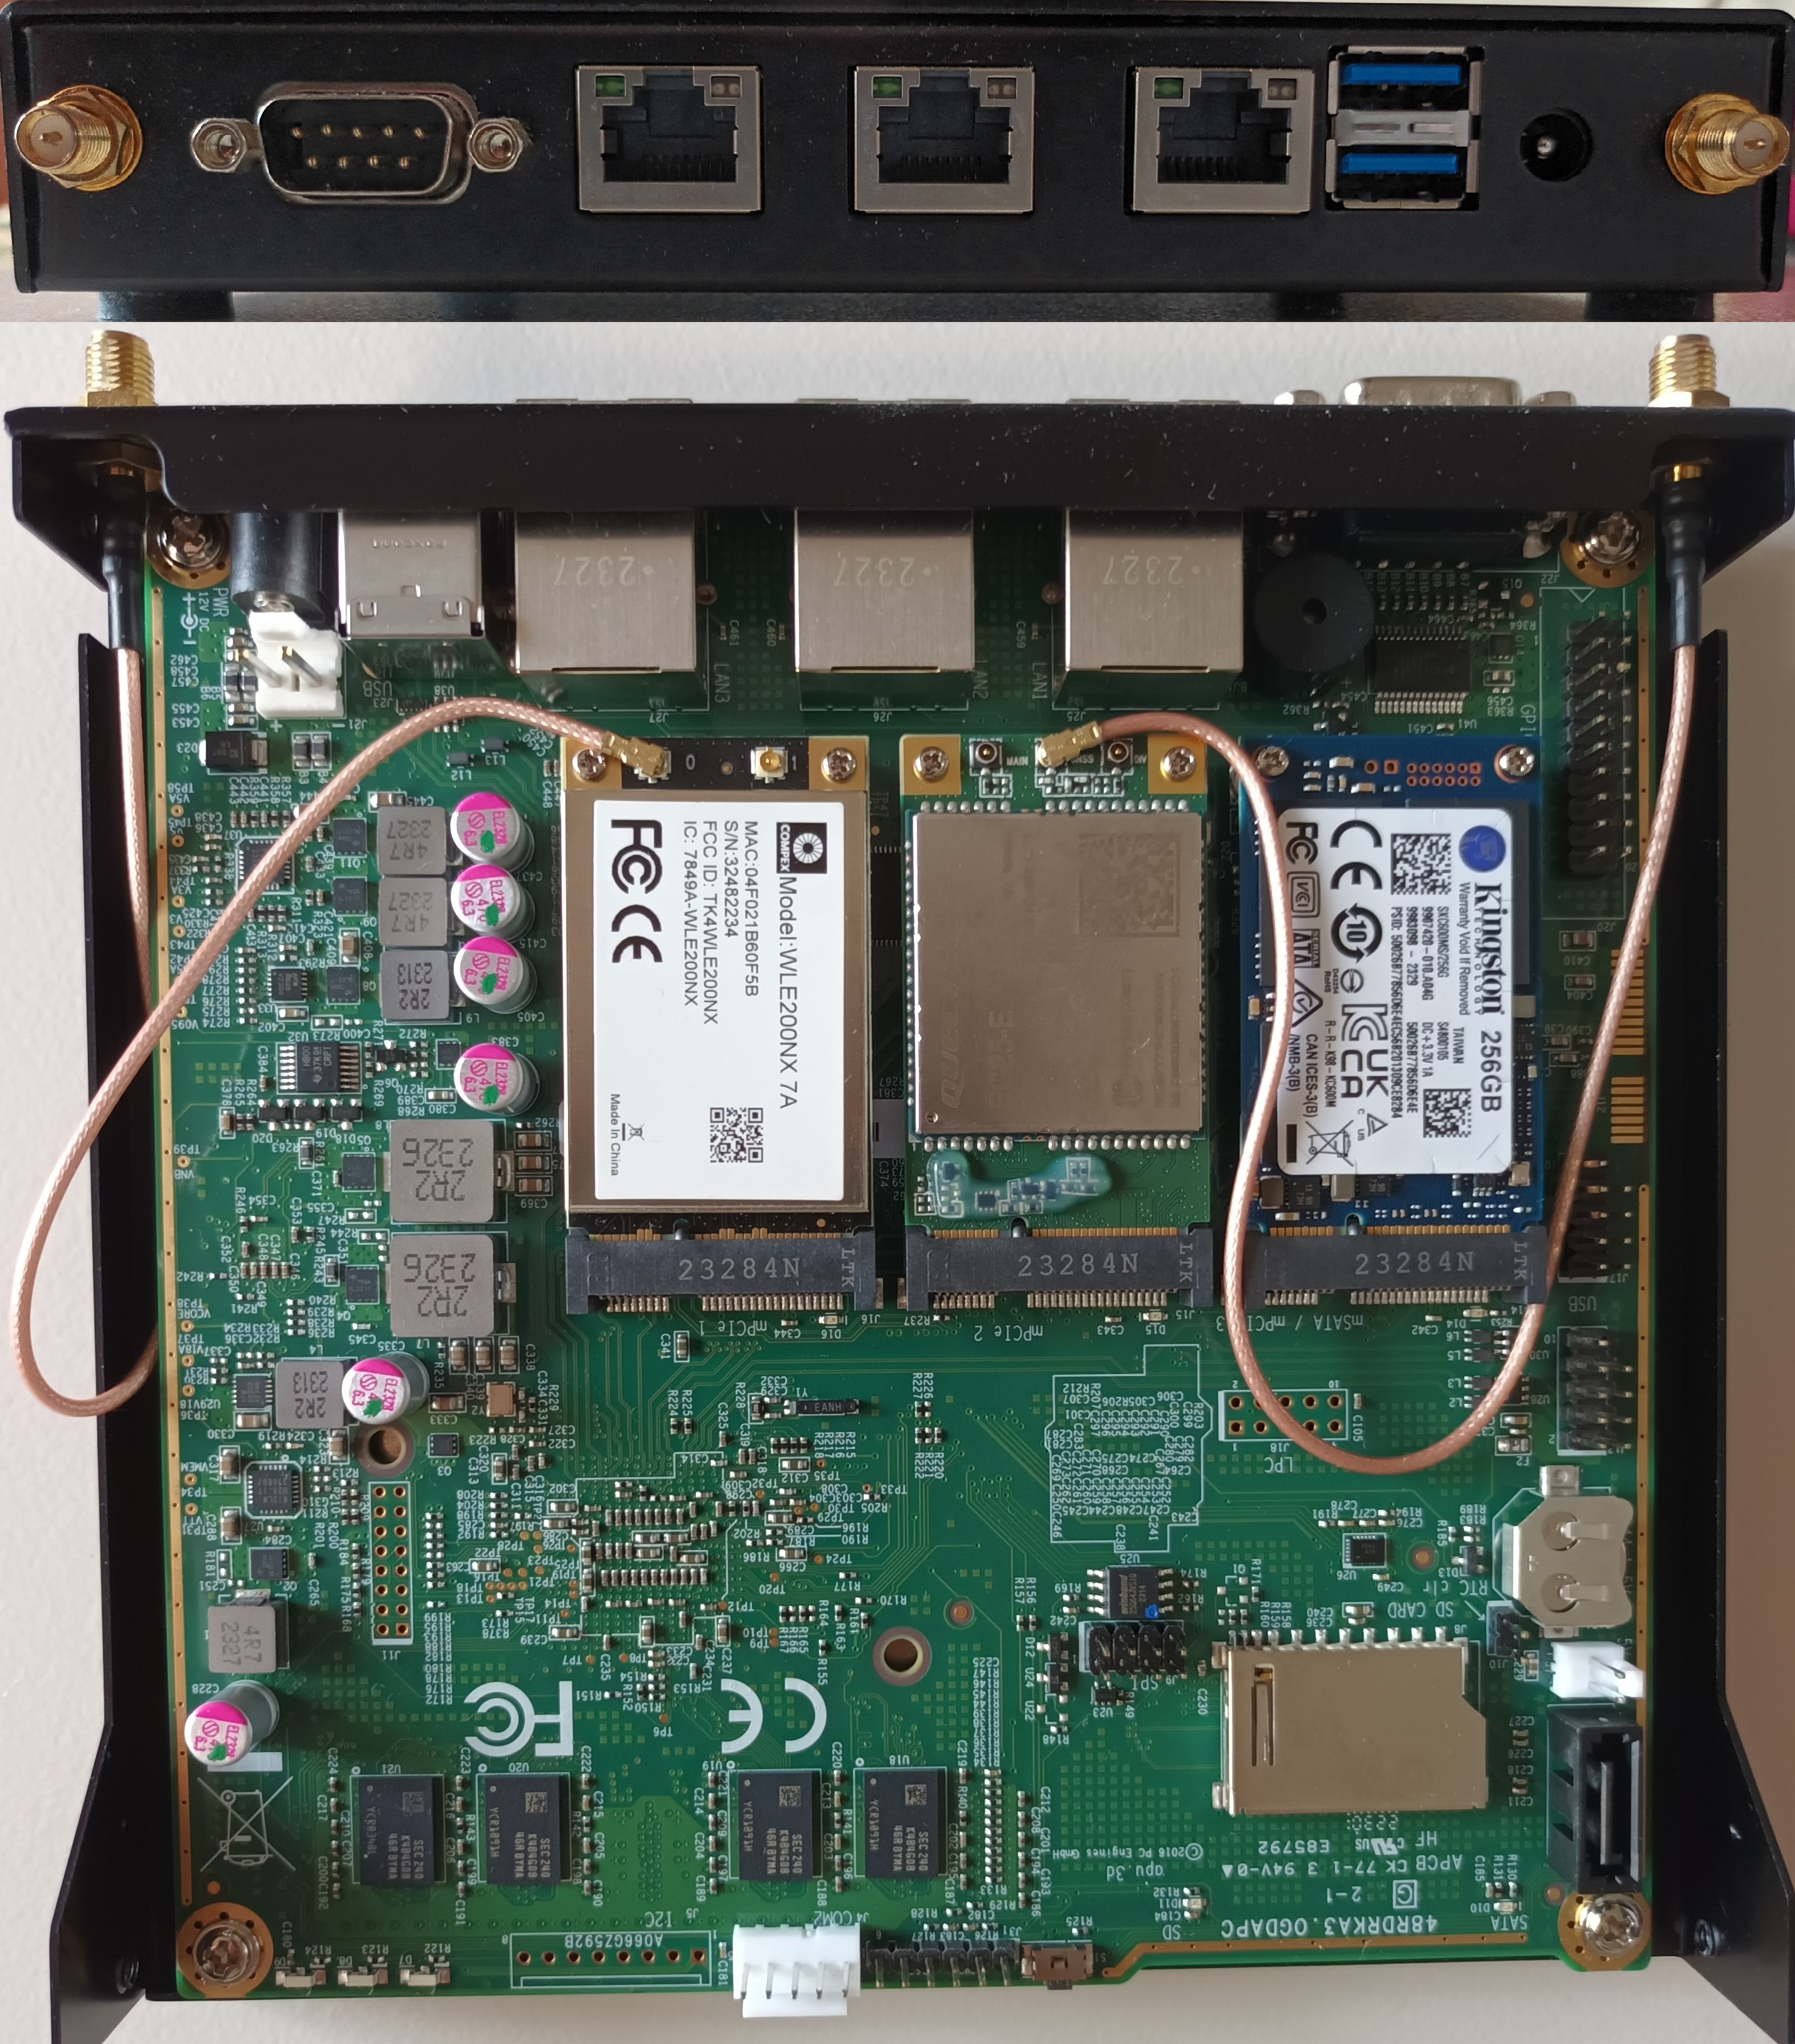
\includegraphics[width=\textwidth]{Chapters/Figures/Implementation/devices/device_1.5.jpg}
	\caption{Back and inside view from device version 2}
	\label{fig:device_2}
\end{figure}


As the device is devoid of any software, we shall adhere to the aforementioned guidelines that have been previously established. It was thus deemed appropriate to proceed with the Ubuntu 24.04.1 LTS, given that the visual interface of the \gls{os} was considered to be of no consequence.
% Fixes to box 2
A minor complication manifested as a result of the incompatibility between the selected WiFi card and the existing solution. During the device setup process, it became evident that, although the WiFi card was from the atheros family, it utilized the ath10k driver. The ath10k driver has been developed as a more recent iteration of the ath9k driver. However, at the time of writing, no patch for \gls{ieee} 802.11p has been made available for this driver. This necessitated the pursuit of a different chip that was compatible with the ath9k driver. Fortunately, the Linux wireless community maintained an up-to-date list of products that met the necessary criteria~\cite{noauthor_external_nodate}. From the list of available options, the Compex WLE200NX 7A was selected as the most suitable choice.

\section[P4/ONOS application implementation]{\gls{p4}/\gls{onos} application implementation}
\label{sec:code}

The technological stack previously delineated and to be utilized in the ensuing tests includes \gls{bmv2} and \gls{onos}. Consequently, it is necessary p4 code for the data plane devices accompanied by Java code for the controller. 

At the outset of the practical component of the dissertation, the original plan was to develop a solution that more closely resembled the \gls{etsi} protocols. However, it was ultimately decided that this approach would not be pursued for two primary reasons. It is first necessary to acknowledge the inherent complexity of the \gls{etsi} protocols. The standards under discussion have been developed over the past two decades by the most esteemed engineers in the field. Given the considerable time and resources required, it is neither realistic nor reasonable to view this as a feasible task in view of the limitations in terms of human resources and time imposed by the context of this master's dissertation. Secondly, the \gls{etsi} norms establish the indispensable presence of the remaining sub-systems as a mandatory condition for attaining the standardized functionality. These circumstances provided the impetus to pursue an alternative and more appropriate course of action. 

In lieu of attempting to create an exact replica of the \gls{etsi} protocol using \gls{sdn} technology, it was elected as more appropriate to pursue the development of a proof-of-concept solution. This proposed endpoint has the dual objective of validating the compatibility of \gls{p4} with wireless interfaces and \gls{ieee} 802.11p, while simultaneously demonstrating the adaptability of \gls{p4} functional capabilities within these specific contexts.
In order to validate the first proposition, the proposed framework will rely on broadcast communication strategies within the wireless domain. The second part will be illustrated through the use of custom headers. While there are numerous potential applications for custom headers, for the purposes of this study, we sought to specify an appropriate research objective. Ultimately, it was determined that the prevention of the perpetual repetition of broadcast messages was a necessary measure to avoid severe network saturation and therefore an appropriate goal. To this end, we created a "marker" system. The markers are unique identifiers generated by the controller and appended to each message transmitted via the wireless interfaces. This strategy guarantees that no message is broadcast twice by the same device. The final solution was developed into a \gls{p4}/\gls{onos} application and the result was published to github~\cite{noauthor_baco-66onos-apps_nodate}.

\gls{onf}, as part of the Aether Project, offers a practical tutorial to teach the fundamental principles of the next-generation \gls{sdn} architecture, which served as the basis for our program. This tutorial was developed for use with Mininet and Stratum, which immediately indicated the necessity for modifications. A more thorough examination of the code revealed the presence of additional issues. It was thus necessary to modify a substantial portion of the code to guarantee its compatibility with the specified environment before it could be utilized. Indeed, a considerable investment of time and effort was necessary to make the program operational.

\section{Summary}
\label{sec:summary}

In this chapter, two implementations were presented, detailing design choices and major requirements. The final box version 2 is the current version in use on other projects. For future reference, the alternatives enumerated in this chapter should be considered for the development of version 3.